\documentclass[border=1pt]{standalone}
\usepackage[T1]{fontenc}
\usepackage{times}
\usepackage{amsmath,amssymb}
\usepackage{tikz,pgfplots}
\pgfplotsset{compat=1.18}
\usetikzlibrary{arrows.meta}
\definecolor{ab}{HTML}{1976D2}
\definecolor{aonly}{HTML}{F4511E}
\definecolor{bcorr}{HTML}{C62828}
\definecolor{ink}{HTML}{263238}
\definecolor{boxfill}{HTML}{F3F7FB}
\definecolor{boxline}{HTML}{90A4AE}
\definecolor{human}{HTML}{F9A825}
\definecolor{proxy}{HTML}{78909C}
\tikzset{
  panel/.style={font=\small\bfseries, anchor=south west, inner sep=0pt},
  stepbox/.style={draw=boxline, rounded corners=3pt, line width=0.5pt, fill=boxfill, align=center,
                  text width=1.92cm, minimum height=1.5cm, inner sep=2pt, font=\footnotesize},
  go/.style={-{Stealth[length=4.5pt,width=3.6pt]}, line width=0.75pt, ink!85},
  cell/.style={minimum size=0.2cm, inner sep=0pt, draw=white, line width=0.6pt},
  note/.style={font=\scriptsize, align=center, inner sep=1pt, text=ink},
  lab/.style={font=\scriptsize, inner sep=1pt},
}
% Item rows: proxy-score cell, then three human-rating cells (#4 = 1: rated; 0: unlabeled).
% #1 x of the left edge, #2 y of the top edge, #3 number of rows.
\newcommand{\itemgrid}[4]{%
  \foreach \i in {1,...,#3}{
    \node[cell, fill=proxy, anchor=north west] at (#1, {#2-(\i-1)*0.22}) {};
    \foreach \j in {1,2,3}{
      \ifnum#4=1
        \node[cell, fill=human, anchor=north west] at ({#1+0.14+\j*0.22}, {#2-(\i-1)*0.22}) {};
      \else
        \node[cell, fill=black!3, draw=black!35, densely dotted, line width=0.4pt, minimum size=0.17cm,
              anchor=north west] at ({#1+0.155+\j*0.22}, {#2-(\i-1)*0.22-0.015}) {};
      \fi}}}
\begin{document}
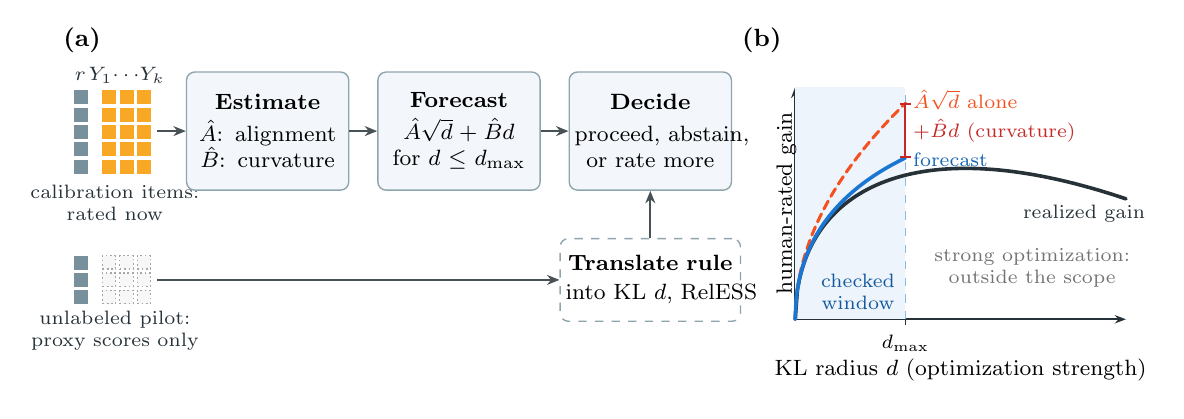
\begin{tikzpicture}
% ---- (a) workflow and information visibility ----
\node[panel] at (0,0.13) {(a)};
\itemgrid{0.12}{-0.32}{5}{1}
\node[note, anchor=base] at (0.22,-0.22) {$r$};
\node[note, anchor=base] at (0.81,-0.22) {$Y_1{\cdots}Y_k$};
\node[note, anchor=north] at (0.66,-1.50) {calibration items:\\rated now};
\itemgrid{0.12}{-2.42}{3}{0}
\node[note, anchor=north] at (0.66,-3.10) {unlabeled pilot:\\proxy scores only};
\node[stepbox] (est) at (2.6,-0.86) {\textbf{Estimate}\\[2pt] $\hat A$: alignment\\ $\hat B$: curvature};
\node[stepbox] (fc)  at (5.03,-0.86) {\textbf{Forecast}\\[2pt] $\hat A\sqrt d+\hat Bd$\\ for $d\le d_{\max}$};
\node[stepbox] (dec) at (7.46,-0.86) {\textbf{Decide}\\[2pt] \mbox{proceed, abstain,}\\ or rate more};
\draw[go] (1.2,-0.86) -- (est.west);
\draw[go] (est.east) -- (fc.west);
\draw[go] (fc.east) -- (dec.west);
% Dashed: needed only when the planned rule is not a raw-score tilt (e.g., Best-of-N).
\node[stepbox, fill=white, dashed, text width=2.15cm, minimum height=1.05cm] (rule) at (7.46,-2.75)
  {\textbf{Translate rule}\\[1pt] \mbox{into KL $d$, RelESS}};
\draw[go] (1.2,-2.75) -- (rule.west);
\draw[go] (rule.north) -- (dec.south);
% ---- (b) schematic local gain law ----
\begin{scope}[shift={(9.3,-3.25)}]
\begin{axis}[
  width=4.2cm, height=2.95cm, scale only axis,
  axis lines=left, axis line style={ink, line width=0.6pt, -{Stealth[length=4pt]}},
  tick style={ink, line width=0.5pt}, tick label style={font=\scriptsize},
  xlabel style={font=\footnotesize, yshift=4pt}, ylabel style={font=\footnotesize, yshift=-6pt},
  clip=false, every axis plot/.append style={line cap=round, line join=round},
  xmin=0, xmax=0.30, ymin=0, ymax=0.34,
  xtick={0.1}, xticklabels={$d_{\max}$}, ytick=\empty,
  xlabel={KL radius $d$ (optimization strength)}, ylabel={human-rated gain},
  samples=150, domain=0:0.30]
  \fill[ab!8] (axis cs:0,0) rectangle (axis cs:0.1,0.34);
  \draw[ab!50, dashed, line width=0.5pt] (axis cs:0.1,0) -- (axis cs:0.1,0.34);
  \node[lab, ab!75!black, align=center] at (axis cs:0.057,0.04) {checked\\window};
  \node[lab, black!55, align=center] at (axis cs:0.215,0.075) {strong optimization:\\outside the scope};
  % Illustrative curves in x = sqrt(d): A = 1, B = -0.8, and a -0.8 d^{3/2} remainder.
  \addplot[ink, line width=1.3pt] {sqrt(x) - 0.8*x - 0.8*x^1.5};
  \node[lab, ink, anchor=north] at (axis cs:0.262,0.172) {realized gain};
  \addplot[aonly, line width=1.1pt, dash pattern=on 3.2pt off 2pt, domain=0:0.1] {sqrt(x)};
  \addplot[ab, line width=1.3pt, domain=0:0.1] {sqrt(x) - 0.8*x};
  \draw[bcorr, line width=0.7pt, {Bar[width=4pt]}-{Bar[width=4pt]}] (axis cs:0.1,0.3162) -- (axis cs:0.1,0.2362);
  \node[lab, text=aonly, anchor=west] at (axis cs:0.104,0.321) {$\hat A\sqrt d$ alone};
  \node[lab, text=bcorr, anchor=west] at (axis cs:0.104,0.276) {$+\hat Bd$ (curvature)};
  \node[lab, text=ab!85!black, anchor=west] at (axis cs:0.104,0.234) {forecast};
\end{axis}
\end{scope}
\node[panel] at (8.62,0.13) {(b)};
\end{tikzpicture}
\end{document}
